% !TeX root = document.tex
% !TeX encoding = UTF-8 Unicode

\chapter{Configuração de Hardware}%
\label{chapter:hardware-configuration}

A plataforma foi desenvolvida para se comunicar com qualquer \textit{hardware}.
A comunicação se dá através de \textit{drivers}, escritos em \textit{Python}.
Isso é possível através do projeto
\href{https://github.com/acristoffers/ahio}{AHIO}.

Alguns \textit{drivers} já estão disponíveis por padrão, mas pode-se escrever
novos \textit{drivers} personalizados. Para isso copie o arquivo do
\textit{driver} do \textit{Arduino}
(\href{https://github.com/acristoffers/ahio/blob/master/ahio/drivers/arduino.py}{GitHub})
e modifique para acessar seu \textit{hardware}. Caso necessário, leia os
comentários em
\href{https://github.com/acristoffers/ahio/blob/master/ahio/abstract_driver.py}{abstract\_driver.py}.

Salve o arquivo em algum diretório em seu computador e inicie o \textbf{moirai}
utilizando o seguinte comando:

\mintinline{bash}{AHIO_PATH="/caminho/para/diretorio" moirai}

A variável de ambiente \mintinline{bash}{AHIO_PATH} funciona como a variável
\mintinline{bash}{PATH} dos sistemas \textit{UNIX}.

Os \textit{drivers} padrão são: snap7, Arduino, GenericTCPIO, Raspberry ou
Dummy. Nessa tela, representada na Figura~\ref{fig:hardware1}, pode-se
configurar o \textit{driver} desejado. Primeiramente deve-se selecionar o
\textit{driver} na lista. Duas seções serão abertas ao selecionar um
\textit{driver}: Configuração e Portas.

\begin{figure}[ht!]
    \centering
    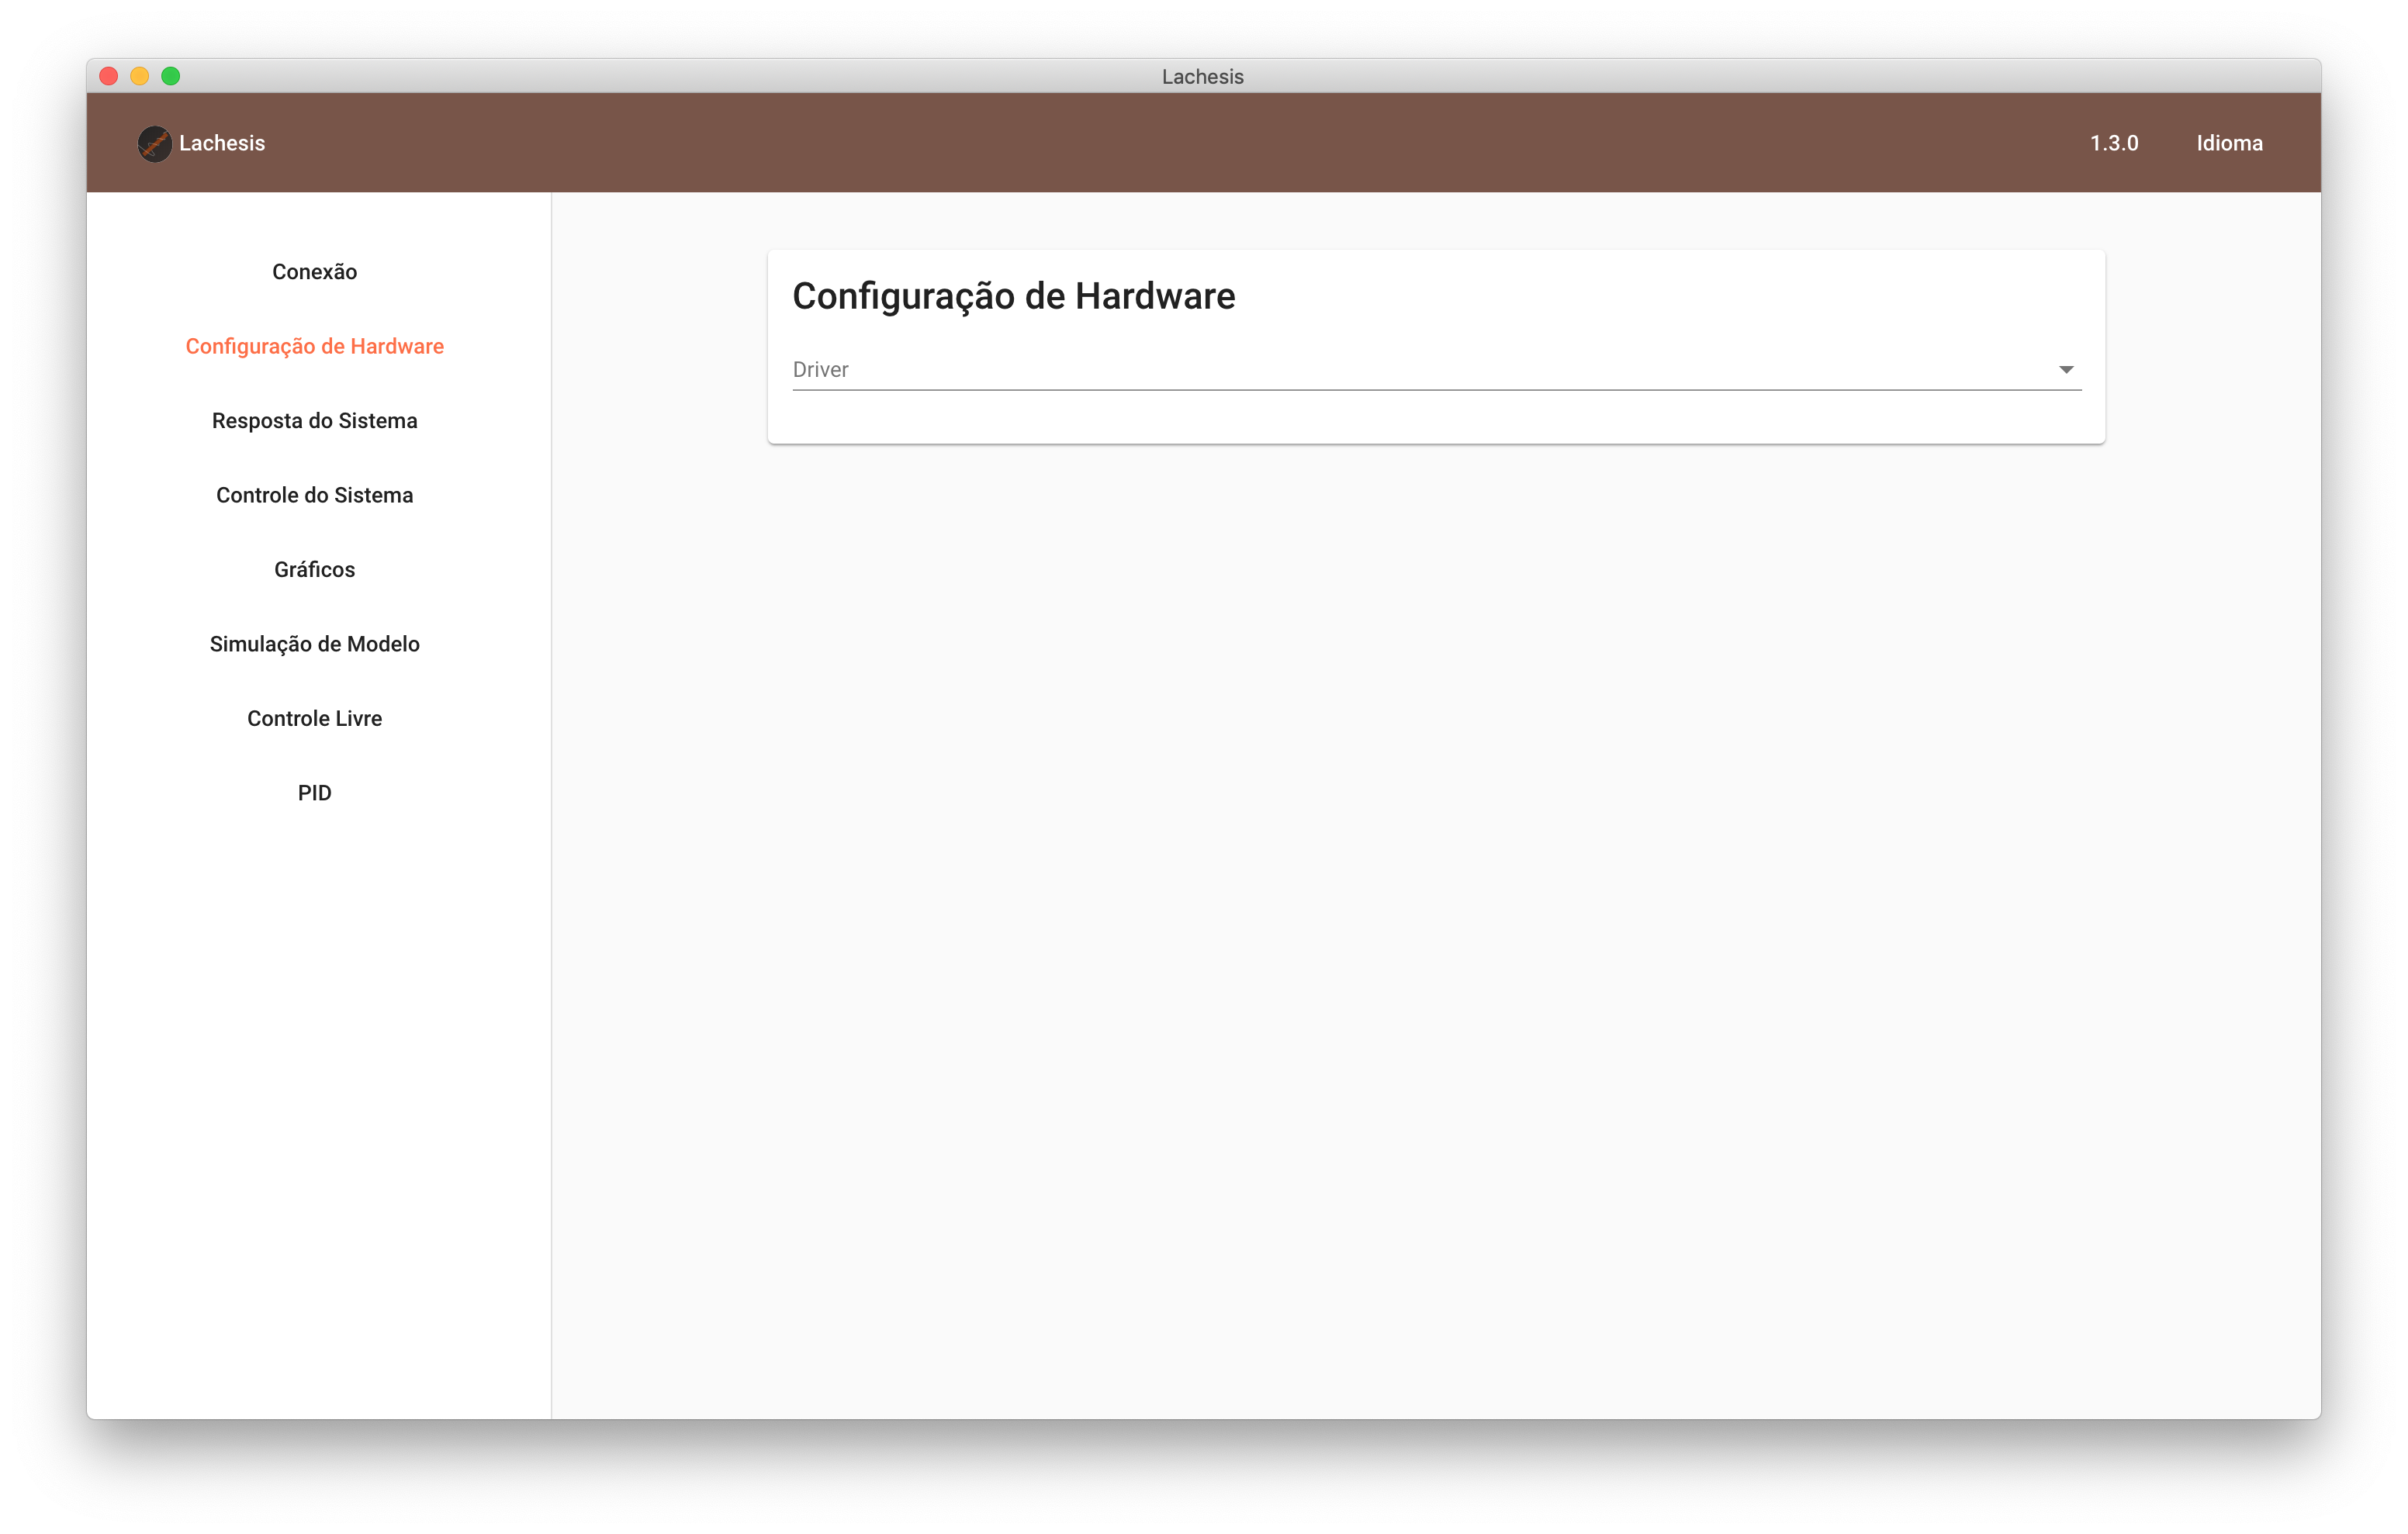
\includegraphics[width=0.9\textwidth]{imgs/hardware}
    \caption[Tela Hardware sem driver selecionado]{Tela Hardware sem driver selecionado}%
    \label{fig:hardware1}
\end{figure}

Na seção \textit{Configuração} deve-se inserir a configuração específica do
\textit{driver}. As opções são os parâmetros do método \textit{setup} quando se
utiliza a biblioteca \textit{AHIO} diretamente. Normalmente serão parâmetros de
localização do \textit{hardware}, como porta do \textit{Arduino} ou endereço do
CLP\@.

\begin{figure}[ht!]
    \centering
    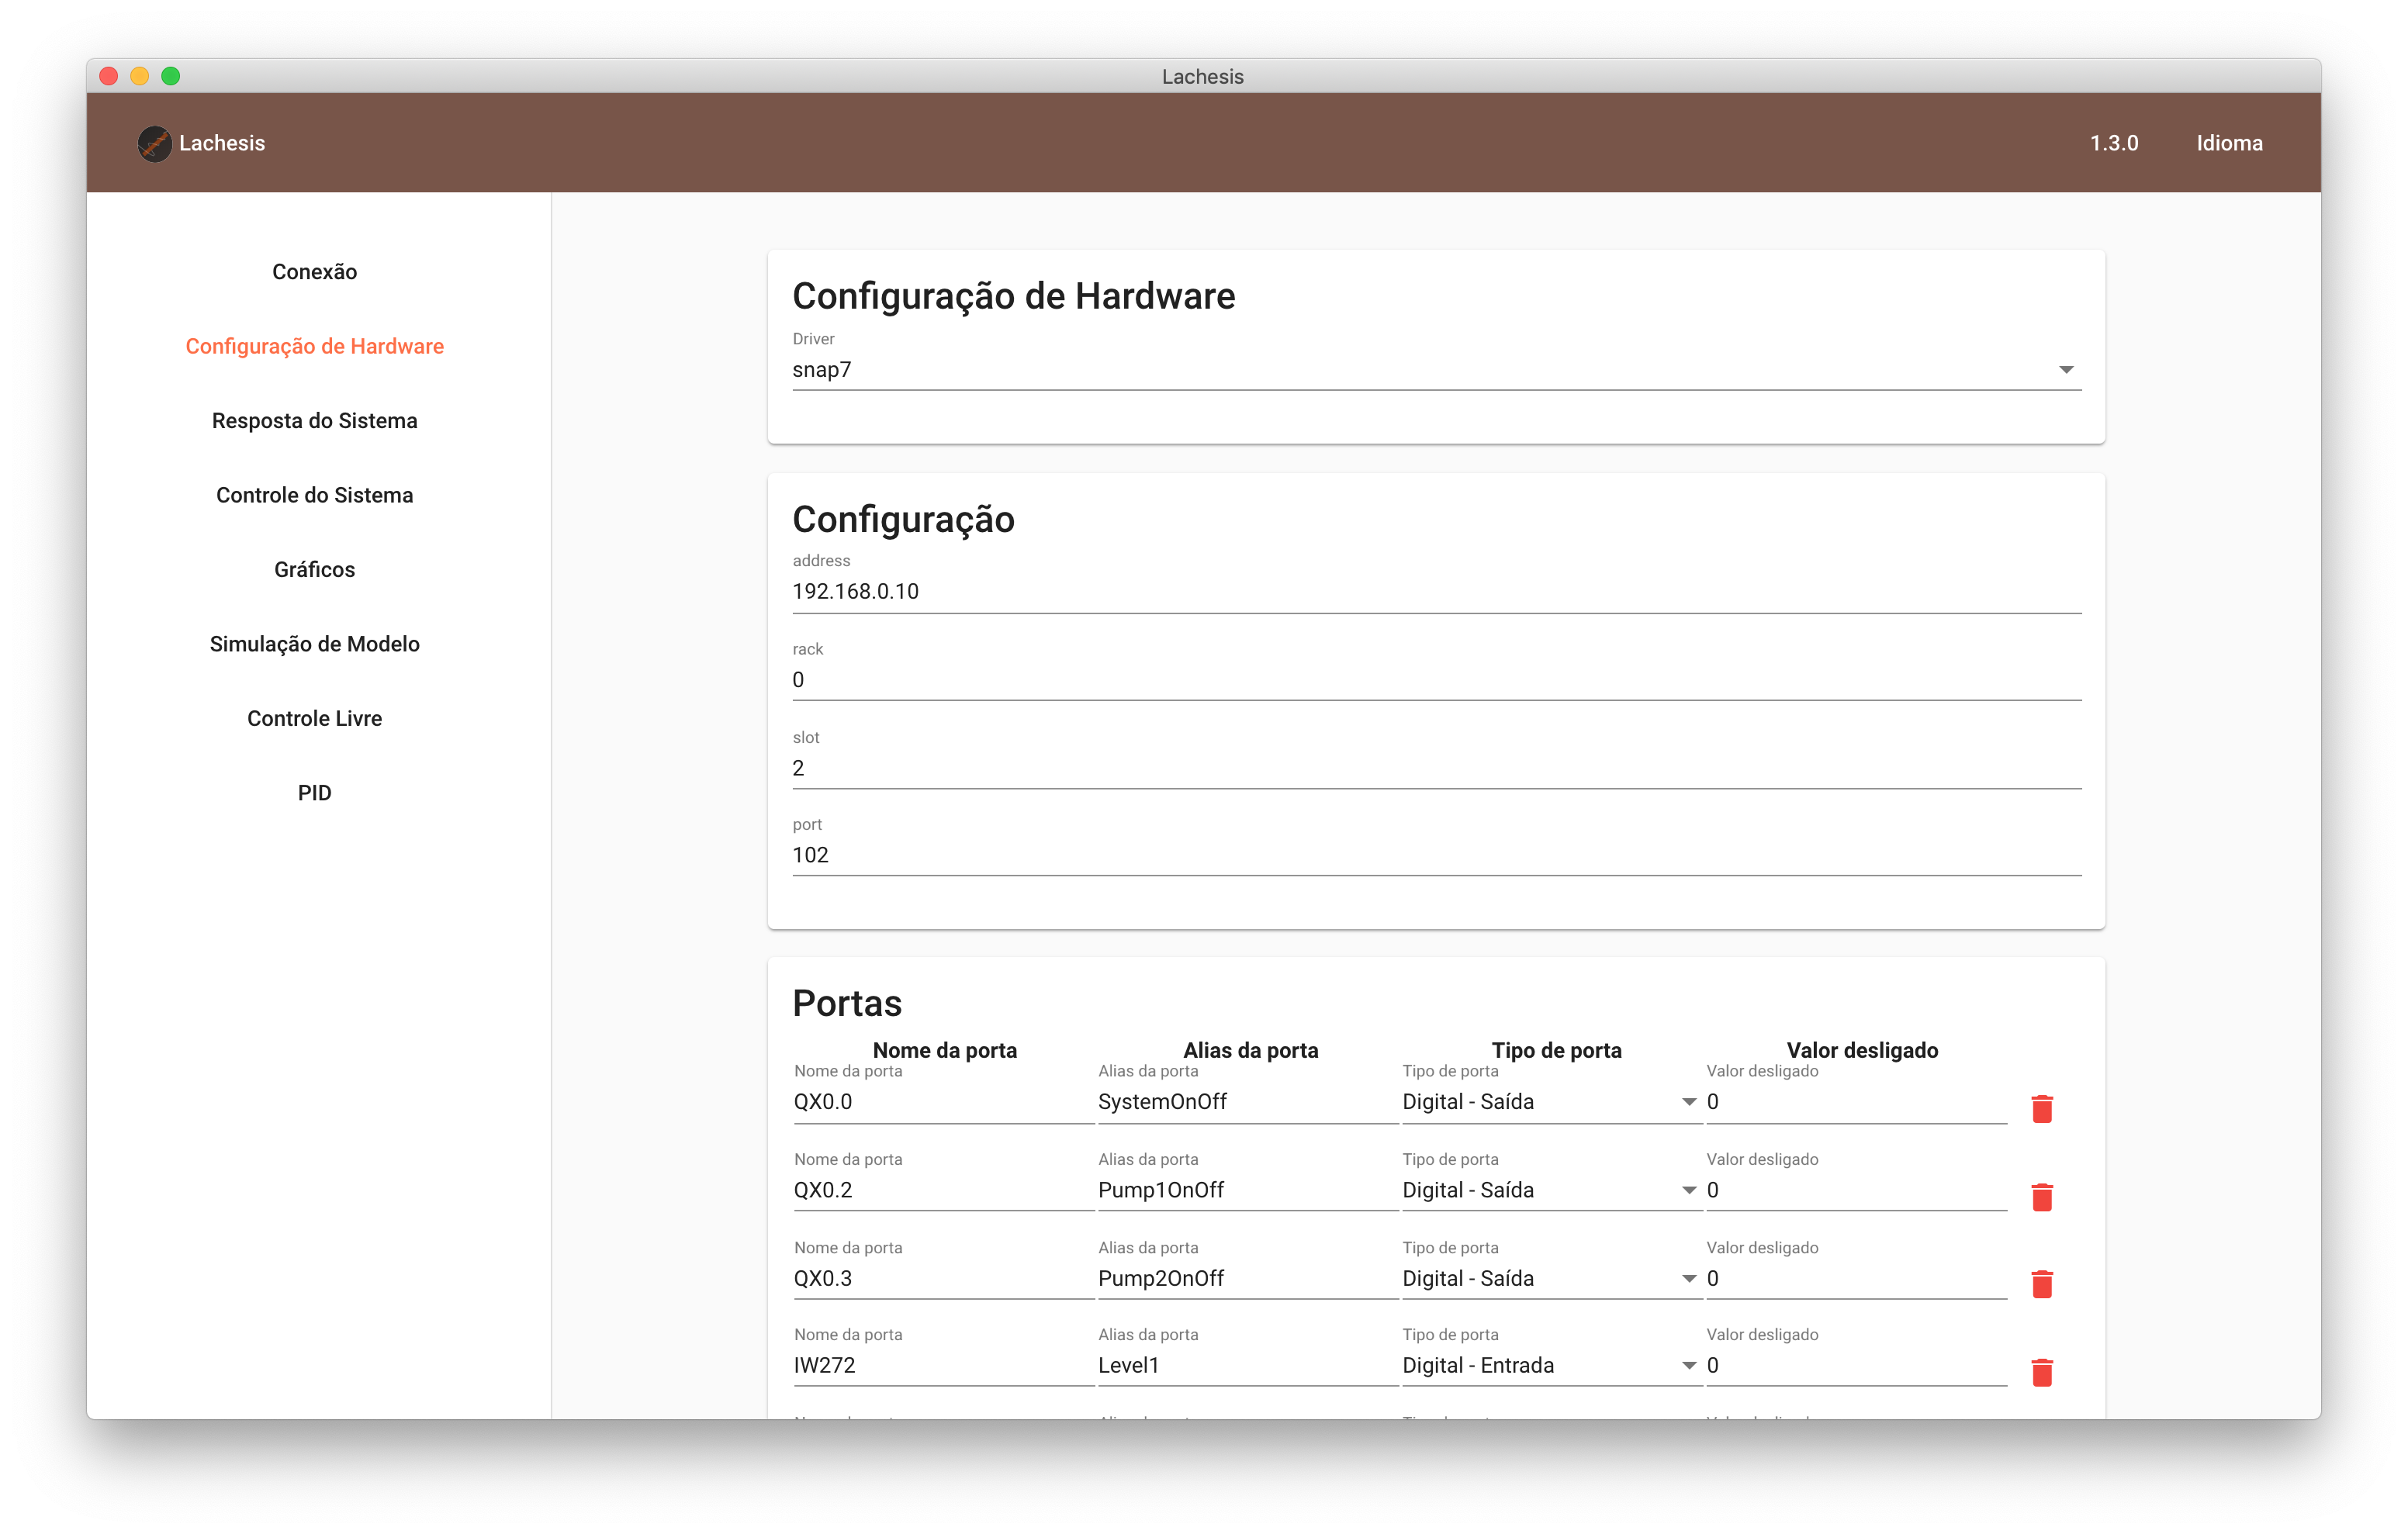
\includegraphics[width=0.9\textwidth]{imgs/hardware2}
    \caption[Tela Hardware com driver selecionado]{Tela Hardware com driver selecionado}%
    \label{fig:hardware2}
\end{figure}

A seção \textit{Portas} (Figura~\ref{fig:hardware3}) permite a configuração das
entradas e saídas do sistema. Ao clicar em \textit{Adicionar} uma nova entrada
em branco é inserida. Ela contém as seguintes colunas: Nome da porta, Alias da
porta, Tipo de porta, Valor desligado.

\begin{figure}[ht!]
    \centering
    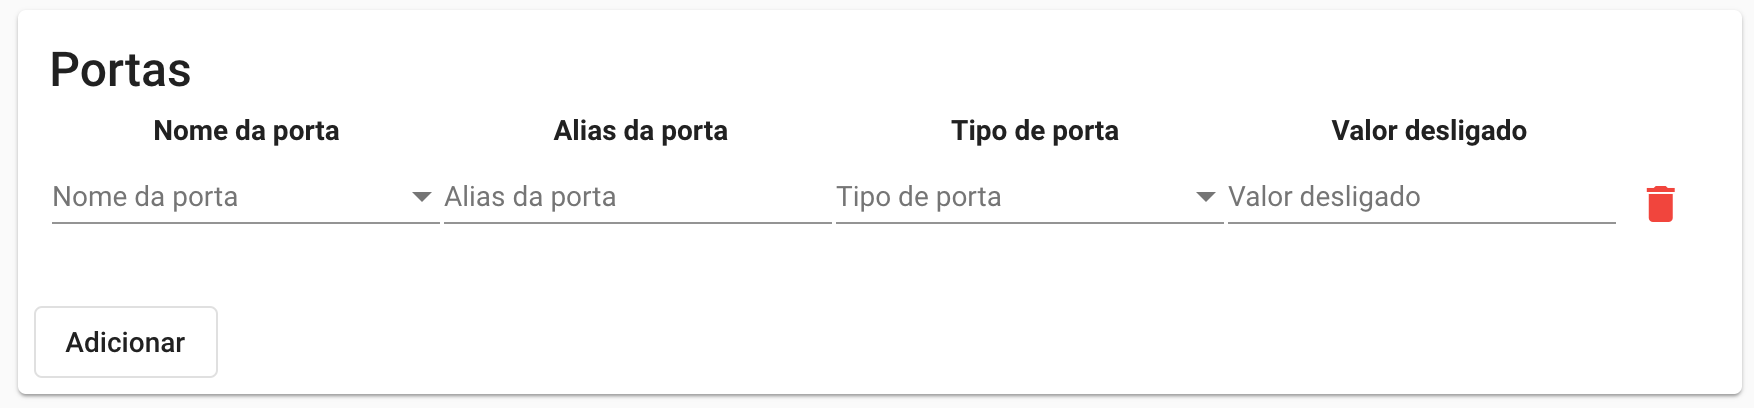
\includegraphics[width=0.9\textwidth]{imgs/hardware3}
    \caption[Seção Portas]{Seção Portas}%
    \label{fig:hardware3}
\end{figure}

O \textit{Nome da porta} pode ser uma caixa de seleção (\textit{dropbox}) ou uma
caixa de texto, a depender do \textit{driver}. No caso do \textit{Arduino}, por
exemplo, será uma \textit{dropbox} com todas as portas do dispotivo. No caso de
um CLP (\textit{driver Snap7}) será uma caixa de texto onde o usuário pode
digitar o nome da \textit{TAG}, como \enquote{QX0.0} ou \enquote{IW292}. Esse
campo referencia a porta física no hardware.

O \textit{Alias da porta} é o nome dado para essa porta física no aplicativo.
Esse nome serve como uma variável e será exibido em formulários e acessado por
código. Escolha um nome que identifique bem o que está ligado à porta. Por
exemplo, num sistema de tanques temos o alias \enquote{Pump1} associado à porta
\enquote{QW272}, pois essa porta irá comandar a bomba número 1 do sistema.

O \textit{Tipo de porta} varia de acordo com a escolha da porta física. Pode ser
uma combinação de digital ou analógica, entrada ou saída. Também pode ser do
tipo saída \textit{PWM}. O \textit{driver} pode limitar as opções disponíveis de
acordo com a porta selecionada.

\textit{Valor desligado} apenas faz sentido para atuadores. É o valor que será
escrito na porta em determinadas situações. Normalmente é utilizado para
desligar o sistema em caso de falhas ou após alguns testes. Se a interface
oferece a opção de definir valores após o teste, essa opção não será usada. Caso
contrário, sim.

Após inserir uma porta, duas novas seções se tornam disponíveis:
\textit{Calibração} e \textit{Intertravamento}.

Na seção \textit{Calibração} (Figura~\ref{fig:hardware4}) pode-se definir curvas
de calibração para as portas. No campo \textit{Porta} deve-se selecionar uma das
portas registradas anteriormente. Note que já são listados os \textit{alias}. No
campo \textit{Alias} deve-se definir um novo nome para a porta. Ambas estarão
disponíveis nos formulários e código posteriormente. O campo \textit{Calibração
estática} permite a definição de uma fórmula matemática que ligue as duas
portas.

\begin{figure}[ht!]
    \centering
    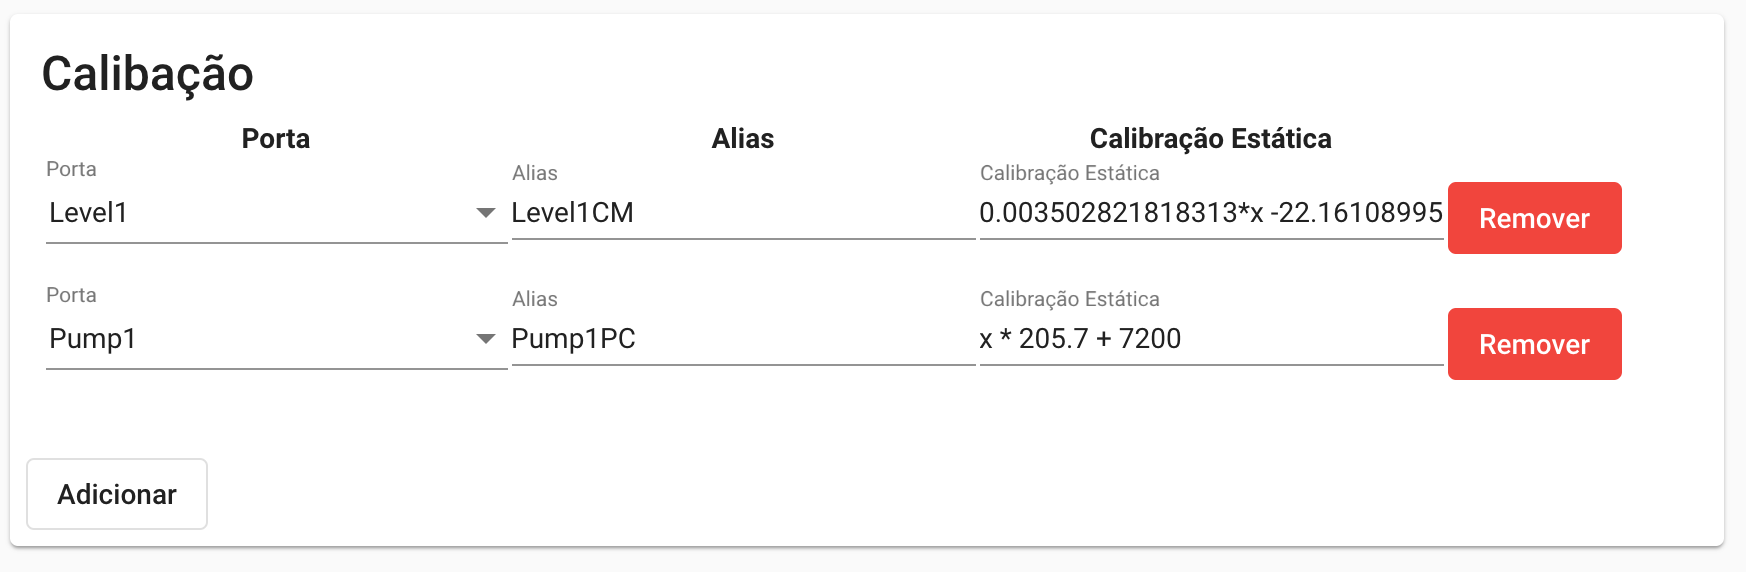
\includegraphics[width=0.9\textwidth]{imgs/hardware4}
    \caption[Seção Calibração]{Seção Calibração}%
    \label{fig:hardware4}
\end{figure}

Como as portas serão ligadas depende se ela é uma entrada ou saída. No caso de
entrada, a nova porta \textit{Alias} recebe o valor da expressão quando se
substitui o valor de x pelo valor da porta selecionada. No caso de saída, o
contrário. Tomando os valores preenchidos como exemplo, temos:

\begin{equation*}
    Level1CM = 0.003502821818313*Level1 -22.161089959823745
\end{equation*}

e

\begin{equation*}
    Pump1 = Pump1PC * 205.7 + 7200.
\end{equation*}

Na seção \textit{Intertravamento} (Figura~\ref{fig:hardware5}) é possível
configurar expressões que, quando verdadeiras, irão definir o valor de outra
variável, além de parar o teste. Exemplo disso é o Intertravamento em um sistema
de tanques comunicantes, caso o nível de água ultrapasse 70 centímetros, o teste
é parado e a variável \textit{SystemOnOff} assume valor zero, desligando o
sistema.

\begin{figure}[ht!]
    \centering
    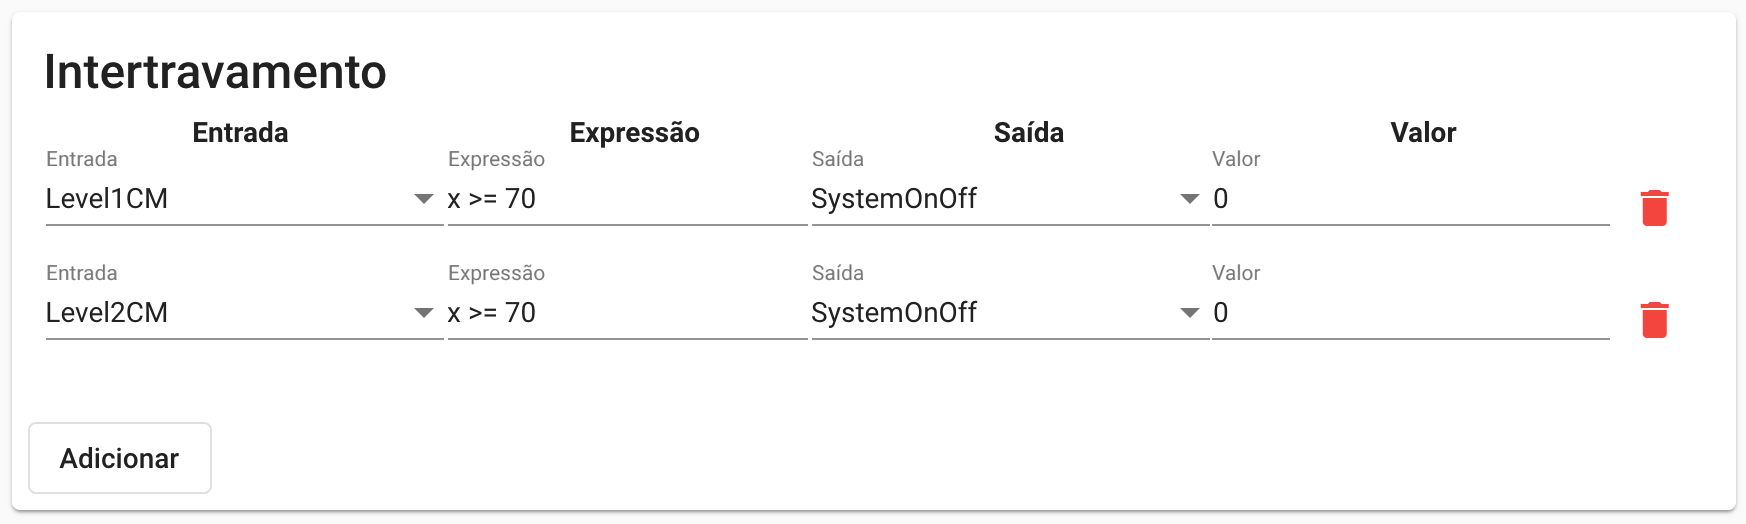
\includegraphics[width=0.9\textwidth]{imgs/hardware5}
    \caption[Seção Intertravamento]{Seção Intertravamento}%
    \label{fig:hardware5}
\end{figure}

No final há opções de exportar/importar configurações de \textit{hardware}
para/de um arquivo, possibilitando o \textit{backup} apenas das configurações do
\textit{driver} ou o compartilhamento de configurações entre pessoas. O botão
\textit{Reinicializar} reinicializa o formulário, sem salvar as alterações. Para
salvar uma configuração nova é necessário clicar na opção \textit{Aplicar}.
Nenhuma configuração será salva se esse botão não for pressionado.
